%!TEX root=../tax-democracy-held.tex
In the preceding \autoref{part:puzzle}, I have tried to shed some light on the \hyperref[chap:3-crises]{threefold crises of welfare, democracy and equality} in much of the current \gls{oecd}-world (\autoref{chap:3-crises}, p.~\pageref{chap:3-crises}).
The puzzle is now a little clearer:

\begin{enumerate}
	\item In spite of unprecendented prosperity, late \gls{oecd} welfare states are less efficient, equitable and sustainable than they could be, because they fall short of an \hyperref[chap:mixed-economy]{ideal mixed economy} (\autoref{chap:mixed-economy}, p.~\pageref{chap:mixed-economy}).
	Among the institutions of the mixed economy, \hyperref[chap:tax-matters]{taxation matters} especially, because it is by far the most effective and efficient tool for government to improve upon, or redistribute market outcomes (\autoref{chap:tax-matters}, p.~\pageref{chap:tax-matters}).

	\item Equipped with a deficient mixed economy and suboptimal taxation, democracies are forced to make unnecessarily unattractive trade-offs between efficiency, equity and sustainability, eroding their \emph{output} legitimacy.
	At the same time, the legitimacy of democratic \emph{inputs} may be undermined by a widening gap between the complexity of an advanced (mixed) economy and the simplifying tendencies of electoral democracy.
	Potentially, pluralist democracy may, in part, have fallen victim to the tightly concentrated special interest that late capitalism offers, especially in the field of taxation.

	Taken together, such diminished legitimacy in outputs and inputs, may help explain widely reported dissatisfaction with democratic performance (but not institutions) \citep[for example,][]{Dalton-2004-aa} and contribute to the apparent mismatch between popular opinion and the governing abstractions of the mixed economy.

	\item Net of such constrained welfare and confused democracy, material and political equality would suffer.
	A deficient mixed economy and suboptimal taxation would corrode the social contract, by which democratic government should have some ability to redistribute the fruits of non-zero-sum %href
	games borne by the free exchange of state-protected property rights \citep[compare][]{Crouch2004}.
	Offered only unattractive choices, and thoroughly confused about the abstractions of the mixed economy, citizens would be increasingly impotent under the social contract.
	One suspects, especially poor and poorly educated citizens would be effectively disenfranchised from the social contract.
\end{enumerate}

\section{Background}
These are, admittedly, conjectures.
As first order actualities, they are puzzling only if there \emph{are} preferable and possible first-order hypotheticals.
%read
	%http://en.wikipedia.org/wiki/Arrow%27s_impossibility_theorem
	%http://en.wikipedia.org/wiki/Gibbard%E2%80%93Satterthwaite_theorem
	%http://en.wikipedia.org/wiki/Unrestricted_domain
	%http://en.wikipedia.org/wiki/Non-dictatorship
	%http://en.wikipedia.org/wiki/Revelation_principle
	%http://en.wikipedia.org/wiki/Voting_paradox
	%https://en.wikipedia.org/wiki/Independence_of_irrelevant_alternatives
	%https://en.wikipedia.org/wiki/Von_Neumann%E2%80%93Morgenstern_utility_theorem


\subsection{Better Taxation}
In the following \autoref{part:tax} (p.~\pageref{part:tax}) and \autoref{part:democracy} (p.~\pageref{part:democracy}), I show that under liberal-pragmatic axioms and orthodox ontology (\autoref{chap:wanted}, p.~\pageref{chap:wanted}), we could have vastly \hyperref[chap:better-tax]{better tax} and \hyperref[chap:better-democracy]{better democracy}.

Among doable taxes, a \glsfirst{pct} potentially supplemented by a \glsfirst{nit}, \glsfirst{lvt} and/or \glsfirst{wt} appears to offer more attractive trade-offs between equity, efficiency and sustainability than the current tax mixes dominated by \glsfirst{vat}, \glsfirst{pit} and \glsfirst{payroll} (see \autoref{fig:ppf-tax-regimes}, p.~\pageref{fig:ppf-tax-regimes}).

%here used to be \ref{fig:ppf-tax-regimes} which is now only in tax-matters

%here used to be \ref{fig:tax-overview}, now only in proposal

\begin{landscape}
 \begin{figure}[htbp]
	\begin{center}
	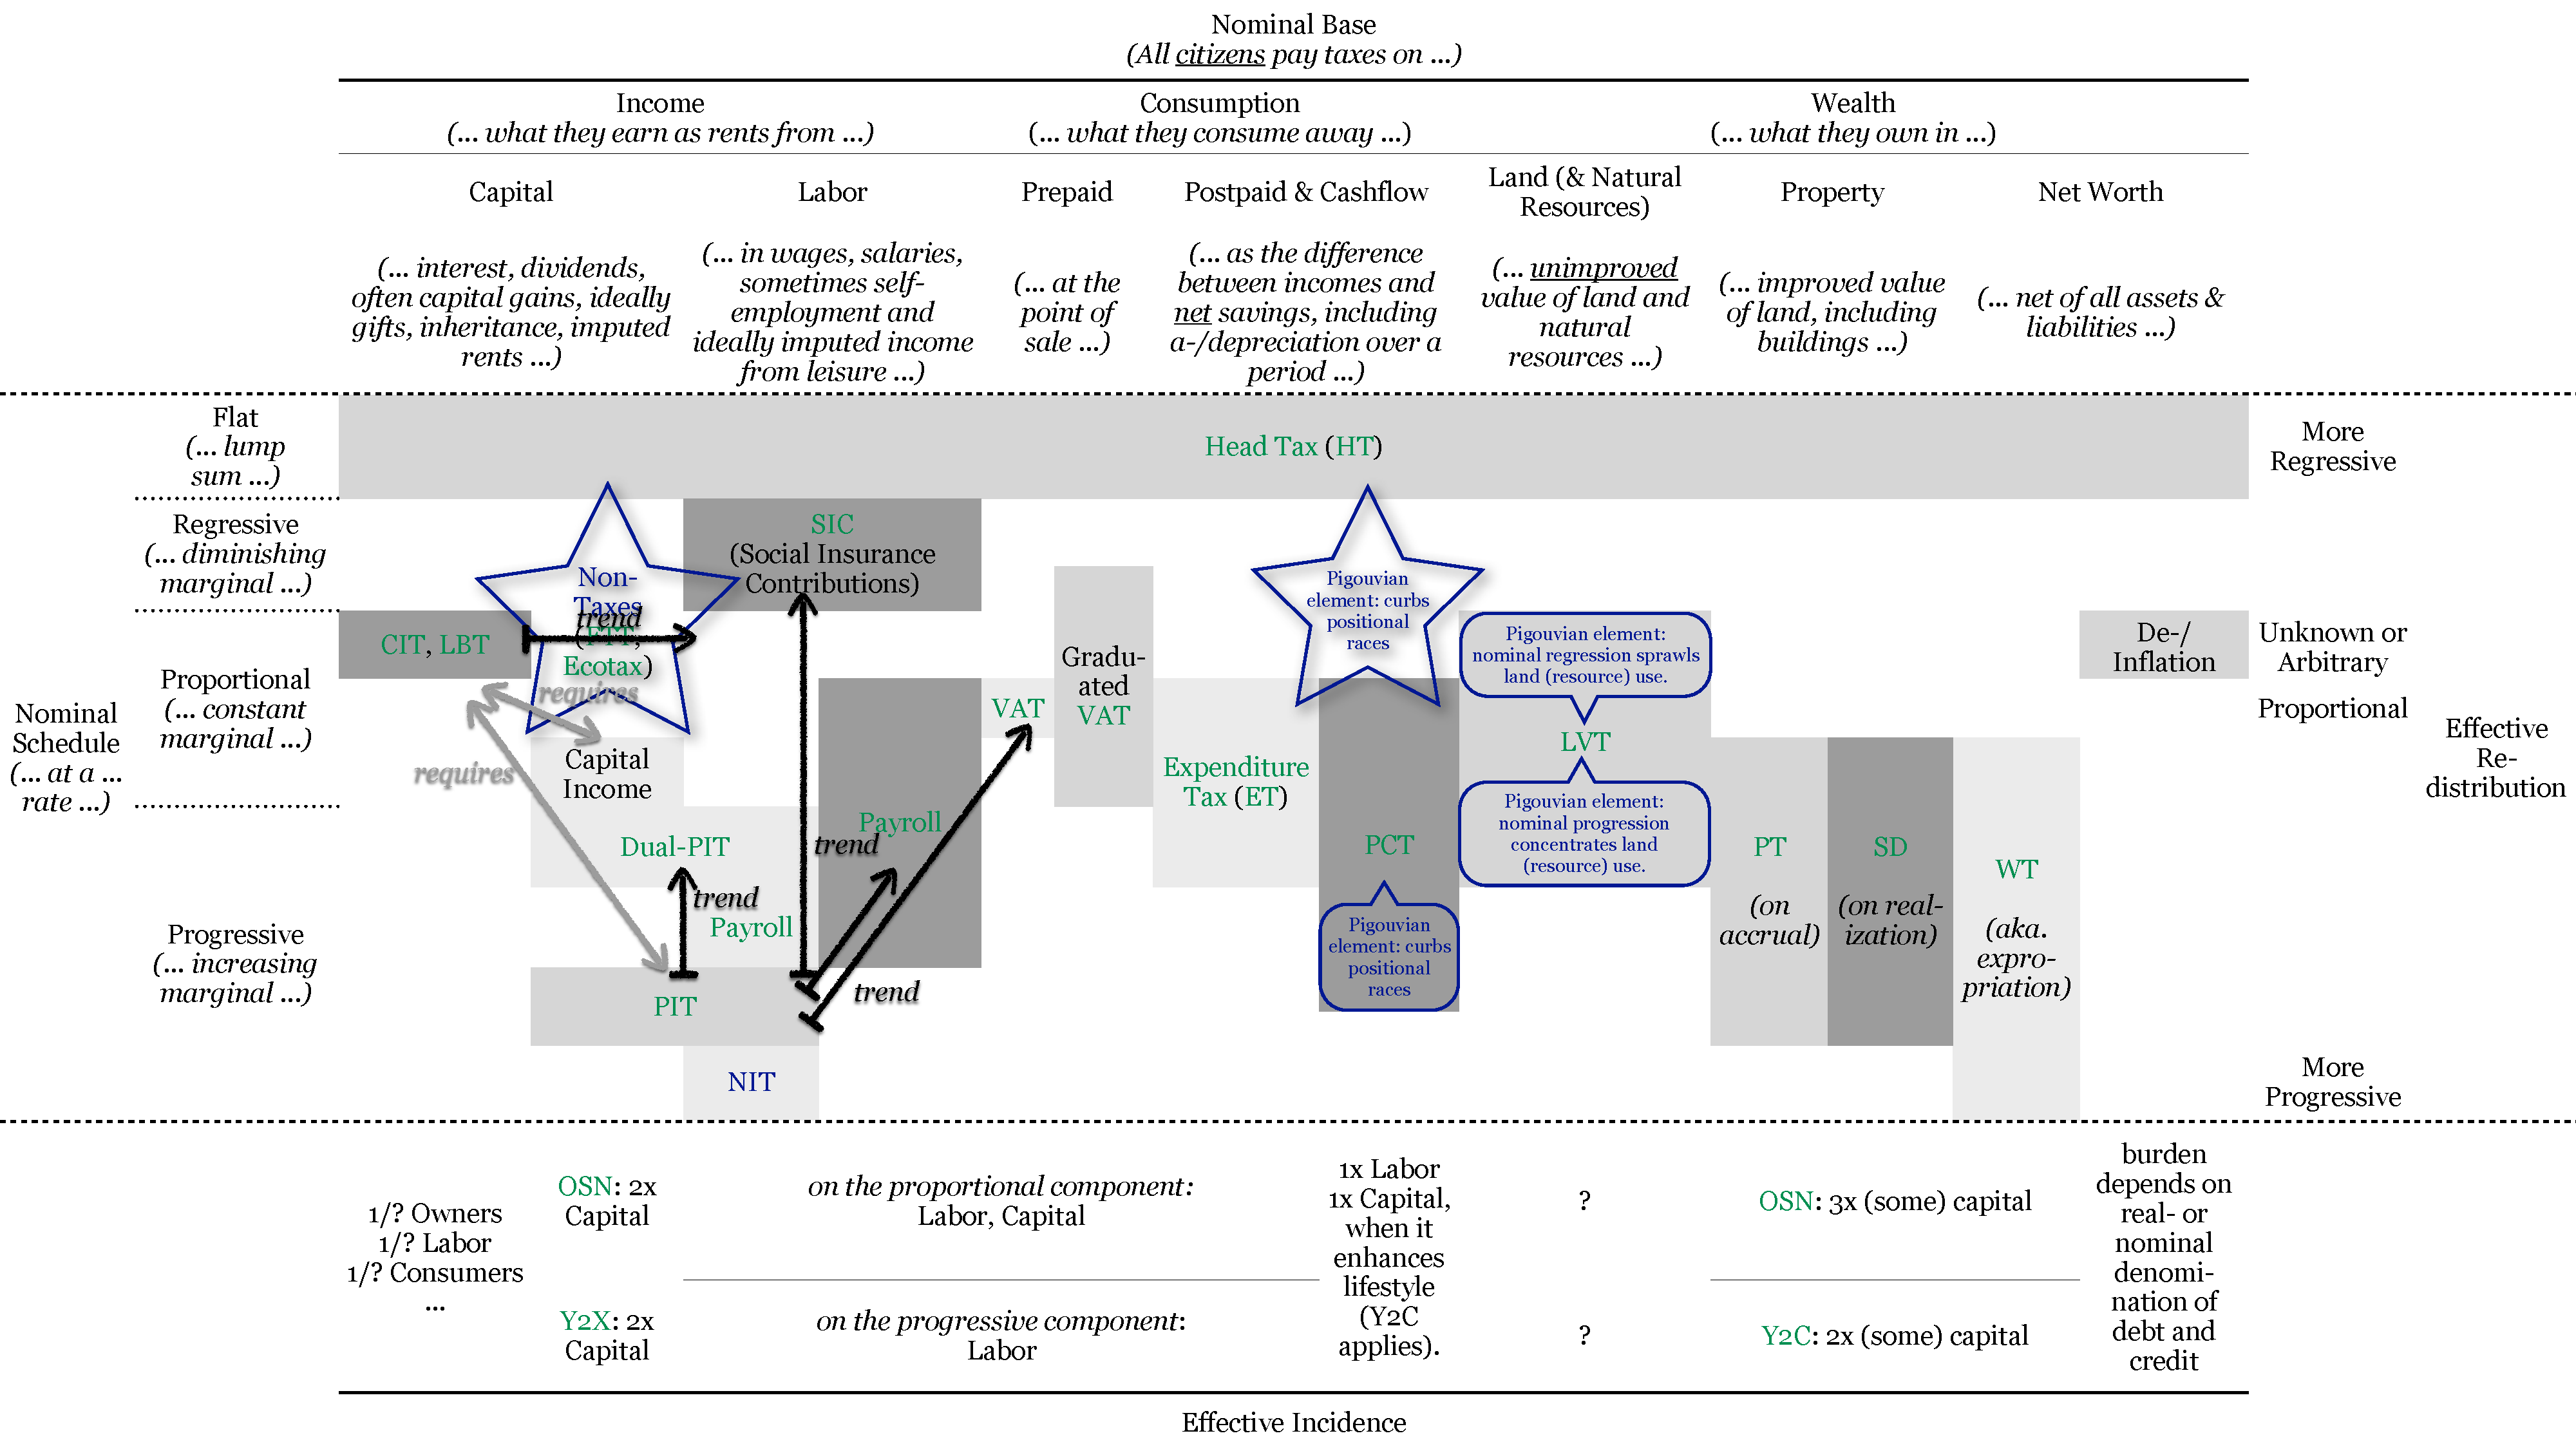
\includegraphics[width=1\linewidth]{tax-with-trends}
	\caption[The Vector Field of Taxes with Trends]{The Vector Field of Taxes with Trends}
	\label{fig:tax-with-trends}
	\end{center}
%	%!TEX root=../tax-democracy-held.tex

\scriptsize{
	\glsfirst{CIT},
	\glsfirst{Dual-PIT},
	\glsfirst{Ecotax},
	\glsfirst{ET},
	\glsfirst{FTT},
	\glsfirst{LBT},
	\glsfirst{LVT},
	\glsfirst{NIT},
	\glsfirst{OSN},
	\glsfirst{PCT},
	\glsfirst{Payroll},
	\glsfirst{PT},
	\glsfirst{SD},
	\glsfirst{VAT},
	\glsfirst{WT},
	\glsfirst{Y2C} and

	\hyperref[sec:distributive-effects-of-inflation]{the distributive effects of in- and deflation} (p.~\pageref{sec:distributive-effects-of-inflation}).
}
\end{figure}
\end{landscape}

\subsection{Better Democracy}
Among doable forms of democratic rule, deliberative democracy \citep[for example,][]{Cohen-1989-aa} appears both more promising and demanding than pluralism.

Deliberation promotes egalitarian, inclusive, well-reasoned and civic-minded discussions for (possibly) consensual political decision-making.
Its normative theory draws heavily on \citeauthor{Habermas-1984}' concept of \emph{communicative action} and \citeauthor{Rawls-1971}' ``Theory of Justice'' as fairness.
Where pluralism encourages the representation of particular interest, deliberative democracy demands \emph{alternative}  conceptions of the common good \citep[18]{Cohen-1989-aa}.
Where pluralism aggregates given, pre-social preferences, deliberative democracy is all about forming preferences.
Where pluralism assumes individual voter error to balance out, when errors are random \citep{Page1993,Surowiecki2004}, deliberative democracy insists on perfecting the deliberators understandings (see \autoref{tab:pluralist-vs-deliberative}, p.~\pageref{tab:pluralist-vs-deliberative}).

%here used to be \ref{tab:pluralist-vs-deliberative}, now only in better democracy
	%it was actually via %!TEX root=../thesis.tex

\begin{table}
	\caption{Pluralist and Deliberative Democracy}
	\label{tab:pluralist-vs-deliberative}
	\small
	\begin{center}
	\begin{tabular}{lcc}
		\toprule 
		 & \emph{Pluralist Democracy} & \emph{Deliberative Democracy}\\
		\midrule
		\emph{Knowledge} & Miracle of Aggregation & Schools of Democracy \\ [10pt]
		\emph{Legitimacy} & Special interest & (Alternative!) Common Good\emph{s} \\ [10pt]
		\emph{Equal Participation} & Representation & Veil of Ignorance \\ [10pt]
		\emph{Speech} & Power & Communicative Action \\ [10pt]
		\emph{Preferences} & Pre-social & Intersubjective\\
		\bottomrule
	\end{tabular}
	\end{center}
\end{table}

Deliberative democracy offers more attractive trade-offs between participation, enlightened understanding and political equality \citep{Fishkin2009} (\autoref{chap:desirable-democracy}, p.~\pageref{chap:desirable-democracy}) and promises to alleviate some of the public choice contradictions of pluralism  \citep[for example,][]{Condorcet1785,Arrow1950} (\autoref{chap:doable-democracy}, p.~\pageref{chap:doable-democracy}).
It also transcends the impoverished, and dubious ontology of pluralism (homo economicus!), and opens legitimate rule to feminist or even virtue ethics.

\subsection{Open Second-Order Questions}
These hypotheticals flow, for the most part, from \emph{a priori} knowledge.
They are grounded in reason, but not --- as hypotheticals can never be --- in \emph{experience}.
I have, as much as possible, supported \emph{a posteriori} assumptions with robust empirical findings --- but I cannot provide  experiential evidence for the complete hypotheticals.

In welfare and tax, comprehensive \emph{a posteriori} knowledge about hypotheticals is hard to come by.

Inframarginal reforms as those I suggest here strain the limits of economic models, all of which must be grounded in only \emph{marginally} known behavioral data.
For example, we would need to know the price elasticity in the demand for luxury goods, or saving and agree on (as I have shown) irreduceably normative judgments of diminishing returns or an optimal savings rate.
%add hrefs
Natural experiments are, of course, unavailable and the external validity of any laboratory setting will be strictly limited.
There is, in other words, not much else beside \emph{a priori} knowledge that we might learn about welfare and tax.
My reasoning here is hopefully as widely agreeable as any comprehensive account of welfare and tax, but it will surely not go uncontested.
Absent empirical clarification, we must then resolve such disagreement in a democratic process.
Taxation, in other words, probably \emph{cannot} be reduced to a first-order question, but it, too reverts to a second-order concern on how to democratically resolve any disagreement we might have about it.
%My topic (tax) is also debated by experts, indeed, experts seem to have the home advantage.
	%But my point is:
%we need to check the work of the experts.
	%ordinary citiznes need to "auf die Finger schauen".
	%We'll see whether the DP or deliberative fora in general can actually do this.

In democracy, we have some, if limited \emph{a posteriori} knowledge about the deliberative hypothetical I here suggest.
Deliberative democracy has been successfully implemented mostly in local settings on policies of limited scope \citep{Fung-2003-ac,HendricksonTucker-2005-aa}.
%not sure this is the right fung reference
In their proposal for ``Empowered Deliberative Democracy'' \citet[17]{FungWright-2001-aa} explicitly suggest what underlies much of the current designs:
\begin{quote}
	\begin{enumerate}
		\item A focus on \emph{specific, tangible} problems

		\item Involvement of \emph{ordinary people} affected by these problems and officials \emph{close} to them

		\item The deliberative development of solutions to \emph{these} problems.
	\end{enumerate}
\end{quote}

Few attempts at deliberating regional issues of greater  complexity have been made, including a `Citizens Assembly' on electoral reform in British Columbia, Canada \citep[confer][]{Ratner-2008-aa}.

On the one hand, deliberative theorists as \citet[17]{FungWright-2001-aa} have criticized this limited scope of deliberative attempts, focused on the immediate, tangible and ``confined to the realm of neighborhood and locale'', as much out of necessity, as out of conviction \citep[759]{Boggs-1997-aa}.
The associated anti-authoritarian, anti-bureaucratic, anti-functional-differentiation impetus may, as \cite{Sousa-Santos-1998-aa} hopes for participatory budgeting in Porto Allegre, Brazil contribute to a ``counterhegemonic globalization'' by concentrating on special issues like land rights, urban infrastructure and drinking water in urban settings, but may by the same token remain ``Bean n' Rice works'' \citep[479]{Sousa-Santos-1998-aa}.
%not the best example, because this is not OECD world
Faced, as our polities inevitably are, with macro-level abstractions, such cherishing of ``human-scale democracy'' above all else may, suspects \citeauthor{Boggs-1997-aa}, move democracy ``in a defensive and insular direction, laying bare a process of conservative retreat beneath a facile rhetoric of grassroots activism'' \citep[759]{Boggs-1997-aa}.
%add somewhere in here:
%an output incongruence arises.

On the other hand, political psychologists as \cite{Rosenberg-2002-aa} have problematized the cognitive demands deliberation poses.
Recent research in political psychology suggests, that --- contrary to the bounded rationality assumption --- imperfect human reasoning may not only stem from remediable cognitive scarcity, but may be developmentally determined.
\citet{Rosenberg-2002-aa} has suggested a threefold developmental sequence and typology of \emph{sequential}, \emph{linear} and \emph{systematic} reasoning.
%add better rosenberg references
His empirical accounts suggest that if any, only systematic thinkers will be able to meet the cognitive demands for reasoned arguments, and egalitarian free speech of deliberative democracy.
Moreover, this cognitive competence was found not to be domain specific, and while people may regress to lower levels of competence under high loads or appropriate cues, they are unlikely to easily, if ever, achieve higher than developed levels.
``Structurally (more and) less developed reasoning adults'' make ``not only the adequacy of citizens' reasoning, but also their \emph{equality}'' a problem for deliberative democracy \citep[12, emphasis added]{Rosenberg-2007-aa}.
%note that the link between rosenbergs sequence thinking and my tax misunderstandings is still to be developed

Few empirical work has been done to address both these ontological and empirical reservations towards deliberative democracy.
We know very little about if and how deliberative fora do in the face of macro-level abstractions and unequally limited cognitive ability of deliberators.

\section{Research Design}

\subsection{Research Questions}

At this intersection of (\gls{pct}) taxation and (deliberative) democracy, two related research questions arise:
\begin{enumerate}
	\item \label{itm:resolve-better-tax}
	Can democratic rule resolve --- and if so, \emph{how} --- any remaining disagreement about \emph{a priori} desirable and doable taxation?

	\item \label{itm:prove-deliberative-democracy}
	Can deliberative democracy address --- and if so, \emph{how} --- the vastly complex, macro-level abstractions facing our polities?
\end{enumerate}

This dissertation investigates the intersecting set of these two research questions.

In on sense, deliberative democracy serves as the \emph{method} to resolve \emph{a priori} disagreement about taxation, and --- equivalently --- to test whether pluralist democracy may be partly to blame for the absence of better taxation.
Deliberative democracy is a good \emph{method} for research question \ref{itm:resolve-better-tax} on taxation, both because I \emph{axiomatize} it to maximize democratic legitimacy, and I \emph{hypothesize} it to reveal some of the dysfunctions of pluralist aggregation plaguing tax choice (see below).
%note somewhere the public choice fuckup

Conversely, taxation is a good \emph{case} to test deliberative democracy in research question \ref{itm:prove-deliberative-democracy}, because it affects everyone, but is shrewd in the kind of macro-level abstractions which deliberative fora have so far avoided
\footnote{
	For this insight, I am indebted to Franziska Deutsch who first noted in 2011 that tax was an interesting case because it affected everyone, but most people knew little about it.
}
and which may strain the cognitive ability of deliberators.

\subsection{Hypotheses}
Both research questions \ref{itm:resolve-better-tax} and \ref{itm:prove-deliberative-democracy} can be rolled up in one set of hypotheses:

%these hypotheses are gone and now in proposal

%here used to be \ref{fig:tax-with-biases} now only in tax-under-pluralism.tex

%here used to be \ref{fig:tax-with-misunderstandings}, now only in proposal

% \citep[334][]{Farrar2010}
	%The present study examines three important hypotheses about deliberation’s effects.
	%The first is that deliberation frequently alters policy attitudes (continuous dispositions towards policy alternatives) – not only at the individual level (‘gross change’) but in the aggregate (‘net change’).
%The second is that deliberation tends to bring policy preferences (ordinal rankings of policy alternatives) closer to single-peakedness, a help in avoiding cyclical majorities of the sort identified by Condorcet and Arrow.
	%The third is that both these effects tend to be stronger for less salient issues, on which less deliberation has already occurred.
	%Since very few issues are highly salient, these hypotheses together imply an important role for deliberation in shaping majorities and making them meaningful.

	%deliberation helps NOT by brining unanimity, but by changing the structure \citep[2]{List2007}

	%here is something important:
%Condorcet works for pairwise comparisons:
%here we got a problem
	% expanded by arrow:
%ANY voting method must violate one of four attractive properties of pairwise majority voting -- which is why it still matters this problem.
%(Fishkin, etal on meaningful democracy:
%1)
	%violations of independence of irrelevant alternatives open the door to agenda manipulation (Riker 1982), strategic voting (Gibbard 1973, Satterthwaite 1975),

	%deliberation increases ``meta-agreement'' on the dimensions of policy, which, in turn decreases the probability of cycling majorities \citep[9]{List2007}

	%also, say \cite[9]{List2007}:
%these should be the REAL dimensions.

	%\cite{List2007} show that you can get more Condorcet winners this way

	%genschel:
%you show that priming works.

	%social choice (Arrow, Condorcet, Gibbard-Satterthwaite), both in \citep[2]{Dryzek2003} and deliberative democracy

\subsection{Methods}

I test these hypotheses by subjecting people to a \glsfirst{dp}, pioneered by James \cite{Fishkin2009}.
This `Gold Standard' of deliberative fora \citep[55]{Mansbridge2010}, combines skillfully moderated small and plenary group discussions of randomly sampled citizens, rigorously vetted, balanced briefings and experts with pre-treatment, post-treatment and control group opinion surveys into a quasi-experimental design (as in \autoref{fig:deliberative-poll-method}, p.~\pageref{fig:deliberative-poll-method}).

\begin{figure}[htbp]
    \centering
	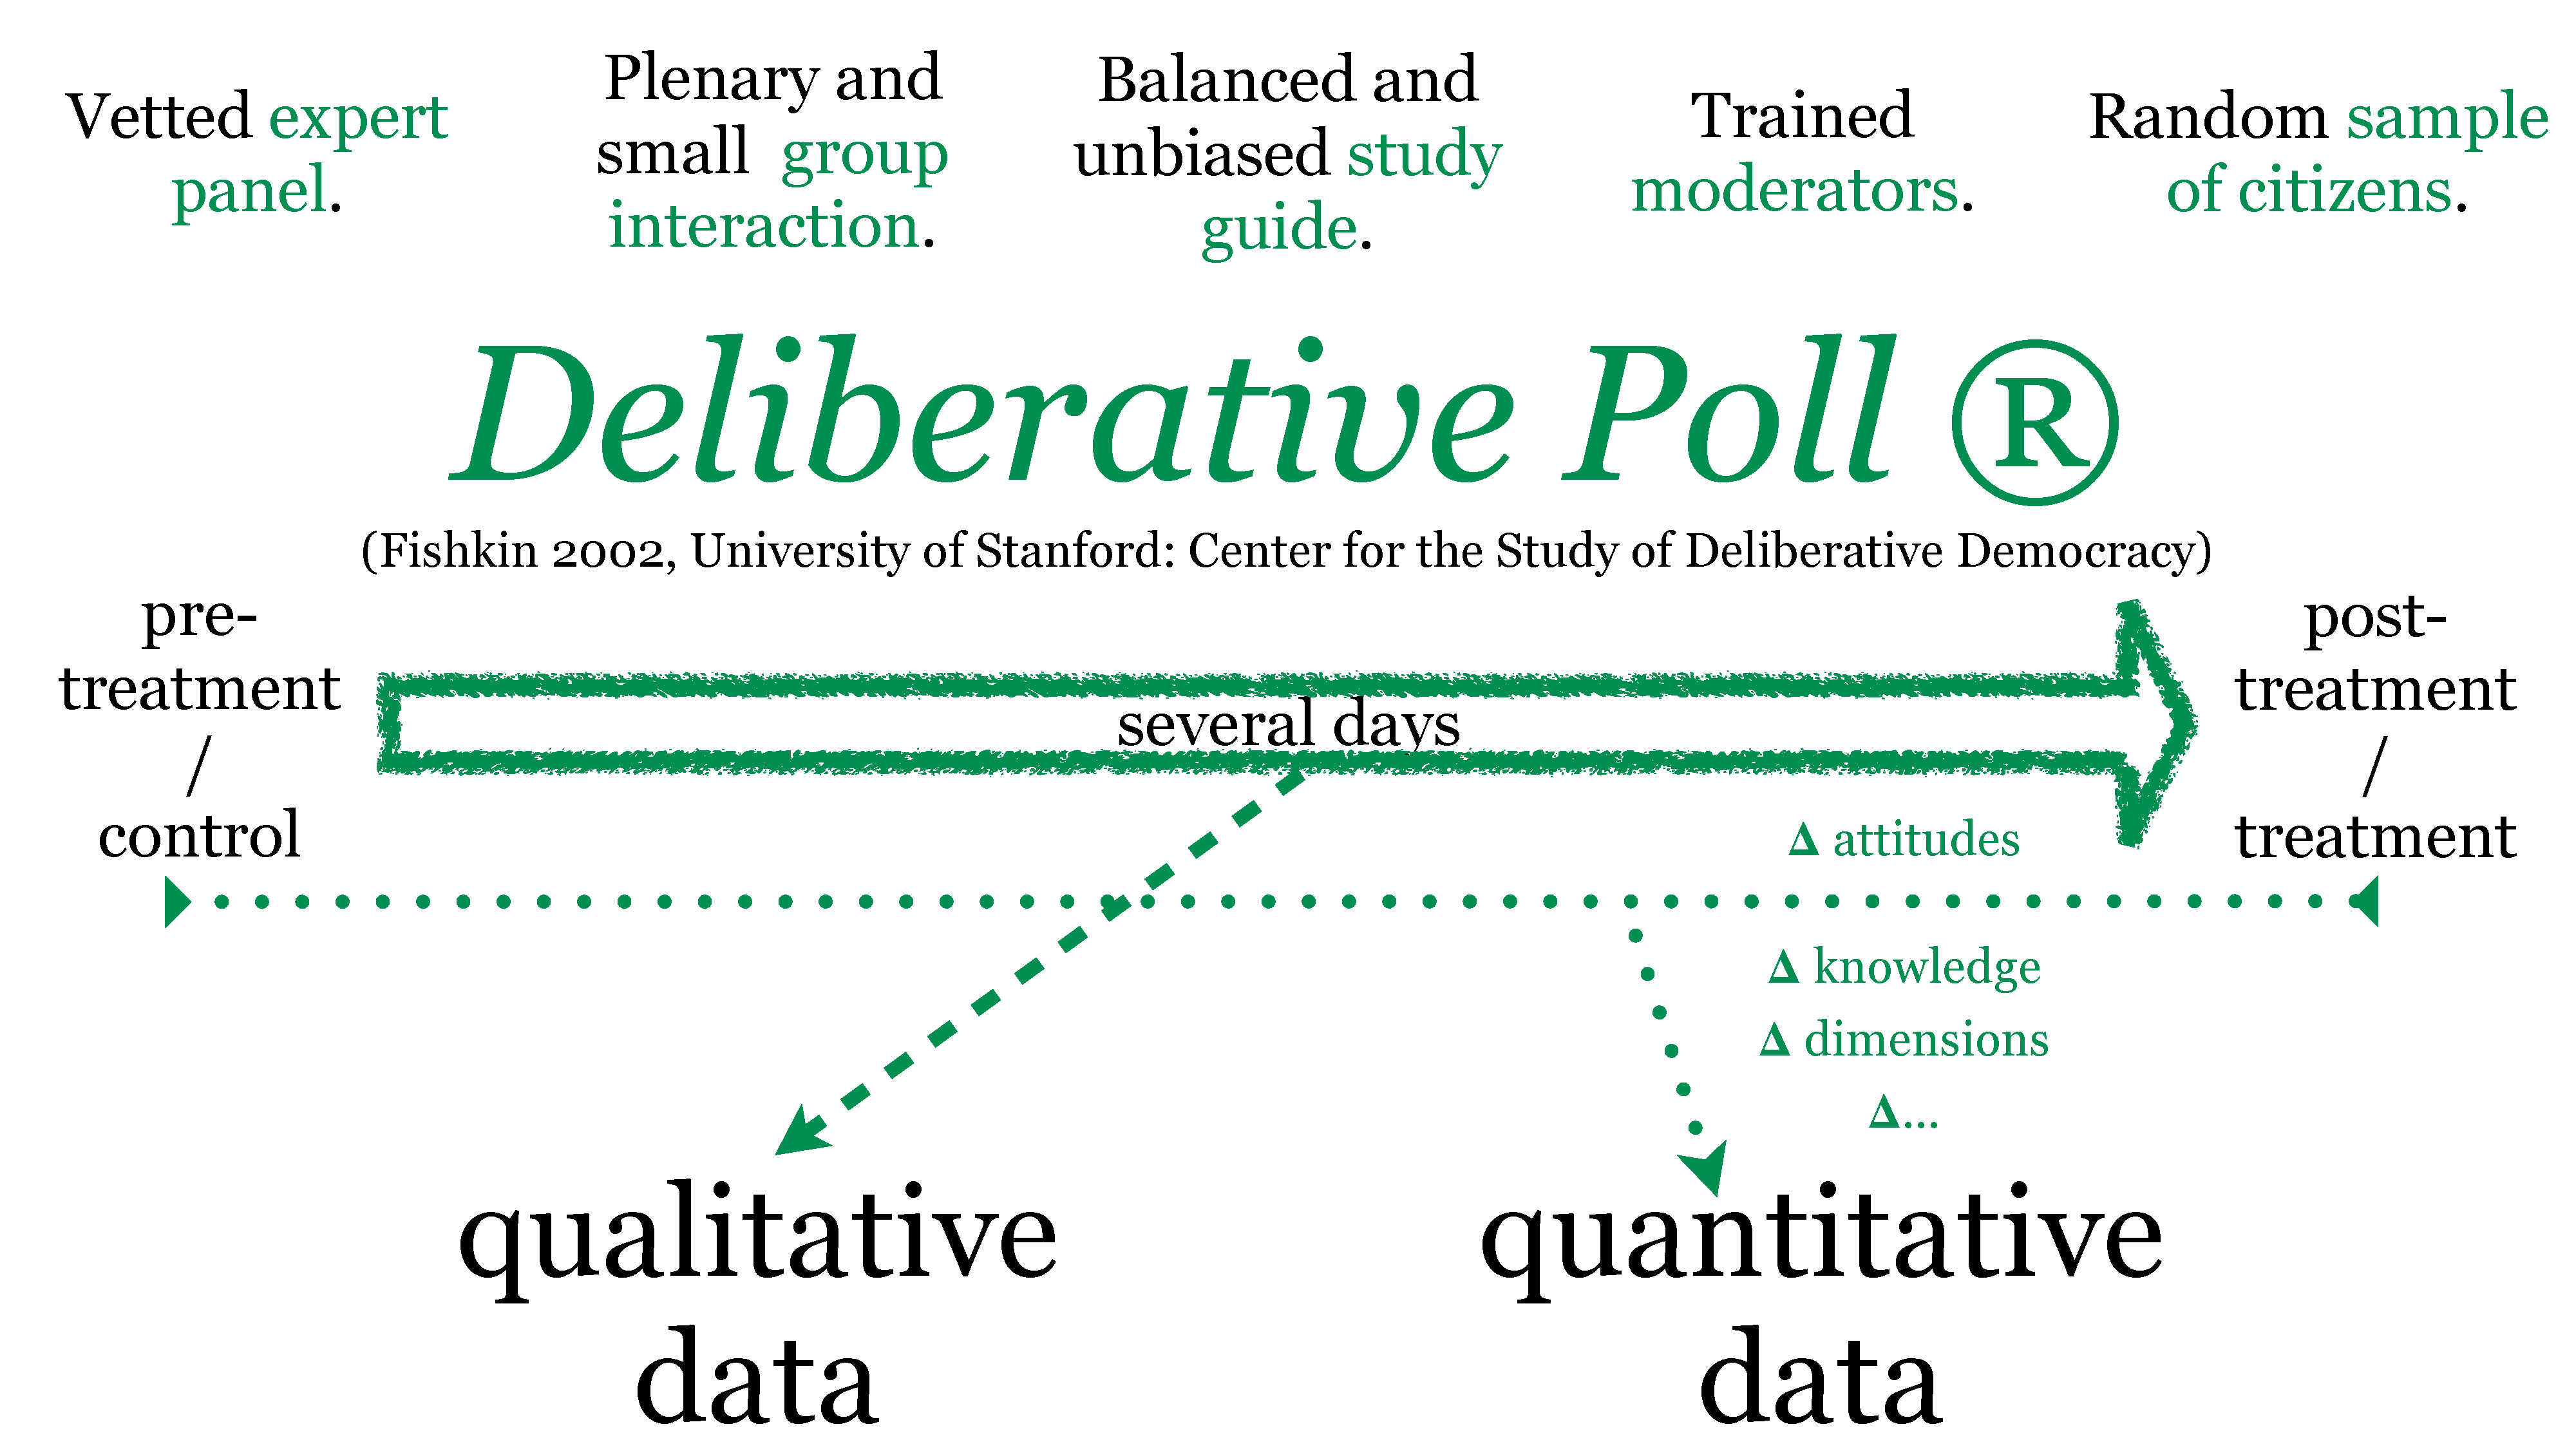
\includegraphics[width=1\linewidth]{deliberative-poll-method}
	\caption{Method of the Deliberative Poll}
	\label{fig:deliberative-poll-method}
\end{figure}

This design suits me well, because it combines the electoral part of democracy with the talking part \citep[308]{ChambersKymlicka2002} and thereby offers the kind of quantitative data needed to test these hypotheses.
Both as a research method and as a second-order hypothetical, it also enjoys high external validity:
it delivers a collective choice and has been shown to work in actual policy making.

	%My thesis investigates this question by qualitatively (discourse analysis?) and quantitatively comparing (survey) the politics (debate) and choice of tax in a status quo pluralist democracy (Germany or the US) with an experimental deliberative forum of ordinary citizens.
	%I hypothesize that ordinary (randomly selected) citizens in a carefully organized deliberative forum will a) think about tax in much greater sophistication, and will b) opt for a PCT regime.

\section{Expected Results}

Hypotheses \ref{itm:knowledge-gain}.x are informed by prior research on the ``Heuristics and Biases in Thinking about Tax'' \citep{McCafferyBaron2003}, supplemented by systematic misunderstandings specific to broad choices between income, consumption and asset taxation.
My hypothesized misunderstandings flow from anecdotal experiences I have had with laypersons and political leaders.
They also shine through in some of the welfare state research, and contrast with my synthesis of an \hyperref[chap:mixed-economy]{ideal mixed economy} (\autoref{chap:mixed-economy}, p.~\pageref{chap:mixed-economy}) and \hyperref[part:tax]{optimal taxation} (\autoref{part:tax}, p.~\pageref{part:tax}).

Hypothesis \ref{itm:attitude-change}, if confirmed, suggests that in fact, remaining \emph{a priori} disagreements about tax \emph{can} be resolved, and that hypothetical taxes really are desirable.

Hypotheses %\ref{itm:preference-structuration}
%something is wrong here!.x
are related to public choice and opinion research in political science, showing that popular beliefs often violate \gls{vnm}-consistence and can fall prey to aggregation dysfunctions.
Opinions about taxation, in particular, may reveal anomalies at the individual and aggregate level, because tax is highly complex and demands highly structured choices.
Past research has shown that deliberation can alleviate preference structuration anomalies  \citep{Farrar2003}.
A \gls{dp} on tax choice might replicate those findings and extend them to another policy area.

Hypotheses \ref{itm:interaction-effects}.x inform the political psychology, both of tax and of deliberation.
If the above effects do not, in fact, interact with equity beliefs (hypothesis \ref{itm:interact-equity}, tax choice must be affected by something \emph{other} than allocative preferences.
In \autoref{fig:ppf-tax-regimes} (p.~\pageref{fig:ppf-tax-regimes}), equity preferences are moves \emph{along} a curve, and shifts or moves of curves reflect preferences orthogonal to equity.
If, as hypothesized, the above effects do not interact with equity preferences, deliberation may reveal (or bring about) popular understandings in line with the suggested institutional \glsfirst{ppf} of \autoref{chap:wanted} (p.~\pageref{chap:wanted}):
If given some thought, people agree that they can shift the trade-off curve between, say, equity and efficiency outwards, and they prefer those institutions that do.
Hypothesis \ref{itm:interact-ses} is broadly related to the post-democracy thesis \citep{Crouch2004}, by which late \gls{oecd} liberal capitalism and democracy not only disenfranchise the social contract, but do so at a socio-economic gradient.
%something is very wrong here, too!
%If confirmed, hypothesis \ref{itm:interact-ses} suggests that under pluralism, people not only prefer taxes less progressive than desired (as per hypothesis \ref{itm:attitude-change}), but that such \emph{false consciousness} is more prevalent amongst people of lower socio-economic status.
The poor (and middle classes) may be too systematically confused to effectively act on their supposed self-interest, reinforcing a mutual crises of political and economic equality.
Lastly, hypothesis
%this does not work/exist anymore!
%\ref{itm:interact-cognitive-ability}
is informed by the political psychology of deliberation, and the empirical research on unequal cognitive ability \citep{Rosenberg-2002-aa}.
If, as hypothesized, people with greater cognitive ability will display greater changes along the aforementioned hypotheses, deliberations on tax, too, may have to consider such unequal abilities in their theory and practice.

%		\section[Enlightened Opinions on Tax (or Research Question)]{Enlightened Opinions on Tax \\(or Research Question)}%Research Question

%			\subsection[Conducting Deliberations (or Methods)]{Conducting Deliberations \\ (or Methods)}%Methods

%			\subsection[Witnessing Deliberations (or Data Collection)]{Witnessing Deliberations \\ (or Data Collection)}%Data

%		\section[Misunderstanding Tax (or Hypotheses)]{Misunderstanding Tax \\(or Hypotheses)}%Hypotheses-1

%		\section[Stretching Democracy (more Hypotheses)]{Stretching Democracy \\(more Hypotheses)}%Hypotheses-2

More broadly, a \gls{dp} on tax choice can inform several fields, including research on public finance and the welfare state, public choice and political economy.

\subsection{Public Finance and Welfare State Research}
If the above hypotheses (especially \ref{itm:attitude-change}) are confirmed, welfare research has a lot more to explain.
If under a legitimate democratic process, people resolve remaining \emph{a priori} disagreements to select a \emph{different} tax than we currently observe, welfare state research must provide a second-order theory of the observed (illegitimate) social choice of suboptimal taxation.
I cannot provide, let alone test that second-order theory of tax choice in this dissertation, but --- if hypotheses are confirmed --- can at least suggest that the democratic forum may be important.
Pluralism may not be the \emph{only} reason why we have no better tax, but it might well be one of several reasons.

Political science and sociology have long tried to explain --- if often implicitly --- tax choice.
At least since the fall of Bretton-Woods in 1972, international tax competition has been at the forefront of the academic debate.
In the extreme form, international tax arbitrage is modeled on a \glsfirst{pd} and Nash-equilibrate at low levels and/or proportional schedules as individual countries compete for mobile capital on global markets \citep[for example,][]{Sinn2004}.
%not sure about the source
This extreme form has garnered relatively little empirical support, and has been modified into more nuanced accounts including country sizes \citep{Piatkowski2008,Genschela}, %not sure about the source
domestic politics \citep{Kemmerling2009}, veto playing \citep{Hallerberg2004} and path dependence \citep{Ganghof2009}.
No matter the independent variable, or its configuration, however, all of this research is plagued by a Panglossian unknown:
to explain just which second-order effect has depressed, or altered taxation you must know how it \emph{could} otherwise be.
If successful, this \gls{dp} may reveal exactly such a first-order hypothetical of taxation.
In the language of game theory and pertaining to the tax arbitrage theory, a deliberatively confirmed tax regime of \gls{pct}, \gls{lvt} or \gls{wt} and \gls{nit} may constitute the social welfare optimum combination of strategies (High / Open), from which the Nash equilibrium may --- or may not --- differ (\autoref{tab:missing-payoff}, p.~\pageref{tab:missing-payoff}).

\begin{table}[htbp]
  \small
   \begin{center}
\begin{tabular}{m{1cm}m{2,3cm}m{2,3cm}m{2,3cm}m{2,3cm}}
& & \multicolumn{3}{c}{\emph{Rest of World}} \\
& &Open Markets $\wedge$ High Taxes & Open Markets $\wedge$ Low Taxes & Autarky  $\wedge$ Any Tax \\
\cline{3-5}
\multicolumn{1}{c}{\multirow{6}{*}{\emph{Home}}} & \multirow{2}{2,3cm}{Open Markets $\wedge$ High Taxes} & \multicolumn{1}{|r|}{?} & \multicolumn{1}{r|}{$x\geq2$} & \multicolumn{1}{r|}{0}\\
\multicolumn{1}{c}{} & \multicolumn{1}{c}{}& \multicolumn{1}{|l|}{?} & \multicolumn{1}{l|}{$x\leq2$} & \multicolumn{1}{l|}{0}\\
\cline{3-5}

\multicolumn{1}{c}{} & \multirow{2}{2,3cm}{Open Markets $\wedge$ Low Taxes} & \multicolumn{1}{|r|}{$x\leq2$} & \multicolumn{1}{r|}{2} & \multicolumn{1}{r|}{0}\\
\multicolumn{1}{c}{} & \multicolumn{1}{c}{}& \multicolumn{1}{|l|}{$x\geq2$} & \multicolumn{1}{l|}{2} & \multicolumn{1}{l|}{0}\\
\cline{3-5}

\multicolumn{1}{c}{} & \multirow{2}{2,3cm}{Autarky $\wedge$ Any Tax} & \multicolumn{1}{|r|}{$0< x\geq$ ?} & \multicolumn{1}{r|}{$0> x\leq2$} & \multicolumn{1}{r|}{0}\\
\multicolumn{1}{c}{} & \multicolumn{1}{c}{}& \multicolumn{1}{|l|}{0} & \multicolumn{1}{l|}{0} & \multicolumn{1}{l|}{0}\\
\cline{3-5}

\end{tabular}
\end{center}
   \scriptsize{The above payoff matrix is not a well-defined, sufficiently formalized game.
To adequately model the international political economy, \emph{Rest of World}, ROW, would have to be disaggregated into at least two more players, making a two-dimensional representation of the game impossible.
Liberalization and taxation are impossible to  be adequately modeled with only two players, for then, autarky of one player would by definition imply autarky of the other player.
In real life, at least theoretically, countries could exit from international trade and finance with other countries still continuing on the road to liberalization.}
   \caption{A Schematic Payoff Matrix for the International Political Economy of Taxation and Liberalization.}
   \label{tab:missing-payoff}
\end{table}

Other areas of welfare state research may benefit from this hypothetical, too.
As I outline in \autoref{chap:tax-matters} and \autoref{chap:hypotheticals-matter}, optimal taxation and an ideal mixed economy matter a great deal as first-order answers to ask the correct second-order questions.
If --- as hypothesized --- people agree that a \gls{pct}, \gls{lvt}/\gls{wt} and \gls{nit} offer more attractive trade-offs between competing values (efficiency, equity), this absence, too is something that welfare state research has to explain.
Here, too, the existing theories rely on such a doable and desirable hypothetical.
The $\Delta$ between that hypothetical and the observed arrangements is a much better dependent variable than spending \citep{Swank-2005-aa} or even decommodification \citep[compare][]{Esping-Andersen-1990-aa}.

%This research informs several fields of \ldots

%	\item{\textbf{International Tax Competition Severely Impairs the Making of Superior Policy}} Specifically, it is hypothesized that indeed --- and counter to the mainstream optimist thesis --- international liberalization \emph{does} restrict the welfare state's ability to redistribute effectively and efficiently (!) as it wishes.
%	\item{\textbf{Veto Playing Matters}} It is hypothesized that veto playing dynamics in particular, and both at the national and international level help explain the suboptimal state of current policy and create a bias for regressive, weak redistribution.
%	\item{\textbf{Tax Harmonization, Development and International Distributive Justice are One}} It is hypothesized that from a careful investigation of the international political economy of tax reform emerges both a political and analytical imperative to think it together with development and international distributive justice.
%Uniformly progressive tax rates on mobile factors of production under the hypothesized hypothetical will crucially affect the chances of developing and emerging markets to capitalize on their comparative advantages.
%\end{description}

%also, hypotheticals are lacking

%Second Order Questions of Social Change
%The second order question of social change is simply:
%Why don’t we have it?
%Possible answers (hypotheses) are:
% Progressive Taxation is subject to an international cooperation problem, akin to a Prisoner’s Dilemma.
%Because the PCT is progressive, it is individually rational for states not to implement it, even if it were collectively rational.
% This is a very interesting question that could potentially greatly enhance our understanding of the international political economy of taxation.
%It however, also requires a comprehensive model of the economy, and even international trade and finance to anticipate the hypothetical payoff of the PCT.
% Tax regimes are subject to great path dependency, they cannot be easily reformed.
% While a historical and tentative analysis of path dependency in tax regimes is possible and probably productive, the costs of reform can ultimately only assessed when a cardinal specification and implementation has been undertaken.
%Assessing the costs of the reform ex ante may be very hard, unreliable or impossible.
%Both a possible international cooperation problem and path dependency in tax regime choice are ultimately endogenous to broader questions of the political economy.
%The cooperation problem depends on the level at which the international political economy is governed.
%Path dependency depends on the domestic and international incidence of reform costs, in turn depending on the states ability to hand out side-payments.

% Ultimately, the PCT could be absent because people do not want it.
%The second order question of social change in tax regimes is:
%will people reject the PCT irrespective of the democratic process that governs their polity?
%If not:
%how do different democratic processes (pluralist, deliberative) constrain or even determine the politics and choice of tax?

%likewise:
%assumed theoretical link:
%if you want to hide injustice, than you'd best do it in a really complex system, like tax.
%
%\subsubsection{Research Question b):
%Why Hasn't it Been Implemented Yet?} Research question b) is then, based on the developed ``perfect tax'', more approximately empirical.
%In the absence of it being implemented in any case, it asks why it has not.
%
%The usual suspect here is a lack of international cooperation.
%Its plausibility will be compared to that of other explanations, namely:
%\marginpar{\textsf{This section needs an overhaul, and \emph{a lot} more reading to make the alternative explanations MECE.}}
%\begin{description}
%	\item{\textbf{Ideology}} Lack of support for such a broadly and boldly redistributive scheme.
%	\item{\textbf{Path Dependency or Historical Institutionalism}} Typological work applies here --- in how far is the tax compatible or not with the institutions and mindsets of established types, for example \cite{BeramendiRueda-2007-aa}.
%	\item{\textbf{Deficient Political Process, Public Deliberation or Discursive Institutionalism}} Literatures on the political process, as well as, on discursive institutionalism \cite{Cerami2009a}.
%	\item{\textbf{International Cooperation Problem}} See above.
%\end{description}

%or addition to science

%First, developed welfare states, in spite of their unprecedented prosperity, appear to be increasingly constrained in their ability to raise revenue and redistribute it as their legislators see fit.
%The pertinent literature on globalization and the welfare state (for an overview see Genschel 2004) asks whether the welfare state has retrenched, and for which reasons.
%Frequently operationalized only as spending (Swank 2005) or decommodification (cf.~Esping-Andersen 1990), that question is incomplete.
%Some of the latently affirmative analyses (Swank 2005) seem to be not so much optimistic about what the welfare state can do, as they seem to be minimal about what it should do:
%income replacement.
%To critically appraise the development of the welfare state, we must instead ask whether legislators are able to raise revenue and redistribute while maintaining growth, factor clearing, low inflation and a positive savings rate.
%We must ask whether legislators were better able to strike this balance of “opportunity and prosperity” (Obama for America, 2007) in the past, or whether there could be a better balance, and then investigate why we do not have better policy.
%Today, welfare states cannot have the cake and eat it.
%They can’t even do one of the two.
%Instead, welfare states are faced with a twin crisis that is mutually reinforcing:
%one of structural unemployment, and one of structural underfunding.
%Structural unemployment is caused by high effective price floors for labor, at or below the socially acceptable minimum income (transfers, minimum wage) in a society, but above the labor productivities of a segment of the workforce.
%Price floors are further raised by an increasingly proportional (or even regressive) tax falling on labor incomes.
%Structural underfunding is caused by a state that is increasingly unable to raise sufficient revenue necessary for the provision of risk pools, public and common goods, as well as to finance its allocative goals.

%Second, my research interest emerges from a sense of utter disconnect between political debate and the abstractions and interests governing the political economy.
%This dis-connect is evident in misleading sloganeering (‘Mehr Netto vom Brutto’, more net out of gross income), widespread superstitions (‘employers [sic!] pay half of social insurance’), bastard Keynesianism (‘consumption is good!’) or redistributive smoke grenades (‘we should tax companies’).
%At a deeper level, I wonder whether pluralist interest and electoral re-presentation can still be reasonably assumed to yield efficient and equitable policies, in an ever more complex world marred by cooperation problems.

%I don't explain the elite-based (potential) reason for the non-reform.
%That, the second-order theory, would be someone elses job.
%discourse theory here?

\subsection{Public Choice and Political Economy}
Public choice has long specified how individual preferences can be aggregated, what it requires and how it can fail \citep[for an overview,][]{Mueller}.
Conversely, (classical?) political economy has formulated theories of how (material?) interest and power can corrupt and alter preference aggregation \citep[for an overview,][]{Robbins1976}.
Both those fields, too, can benefit from deliberating hypothetical taxes.

Public choice, for once, is mostly an \emph{a priori} and often an insular enterprise, merely chronicling --- but not explaining --- the inconsistent preferences and structuration anomalies it faces.
For example, portfolio theory clearly differs from observed loss (not risk!) averse strategies \cite{Kahneman2011}, but we know relatively little about how culture or institutions mediate this gap.
Deliberation is one (possibly attractive!) institution to narrow the gap between \emph{a priori} public choice and \emph{a posteriori} policy preferences.
The hypotheses tested in this \gls{dp} on taxation problematize the institutional link between optimal and actual choice.

Public choice is also hard to bring to bear on real-life political choices, because it deals in such high abstractions and the very consistency in preferences it demands are often subject to (second order) controversy.
It can be difficult to argue how any particular policy may be explained by, or differ from a theory of public choice, as long as there is disagreement over possible alternatives and ontological concepts.
This dissertation synthesizes and develops consistent preferences on taxation, and puts them to a deliberative test.
If successful, it may provide an insightful, practically relevant case study of policy and help resolve the controversy over preferences.

Conversely, (classical) political economy can gain from a \gls{dp} on taxation, because it, too, facing disagreement over alternatives and material ontologies (\citeauthor{Keynes1936} vs \citeauthor{Hayek1931}, as in \citealt{Wapshott2011}), too often reverts to second-order theory, sometimes getting lost in an unproductive muddle of ideas \emph{and} interests, rather than one \emph{or} the other as independent variable.
\footnote{
	Ideational perspectives surely are important, and rationalist epistemologies not the only way to knowledge, but, as I explain in more detail in \autoref{chap:wanted} (p.~\pageref{chap:wanted}), first-order alternatives must be clarified first.
}
This dissertation develops a --- hopefully --- agreeable material ontology for the mixed economy (\autoref{chap:wanted}), and synthesizes a desirable and doable alternative which is then subjected to a specific, legitimate second-order process:
deliberation.
By comparing cognition --- or ideas (!) --- as a \emph{function} of this second-order process, and by relating it to socio-economic outcomes and conditions of deliberators, this dissertation also tests one specific theory of the political economy.
Based on transparent, indeed quite orthodox assumptions, I hope to show that material interest may, through whichever agency or structure, have found a clever way to corrupt democratic rule without resorting to crude power.
If confirmed, my hypothesis suggest that --- for whatever reason --- people systematically misunderstand tax in a way that favors the rich, and more generally, the benefactors of the status quo.

\section{Conclusion}
In Schumpeter's %correct source?
thundering words, taxation and democracy \emph{are} the two sides of social contract (\autoref{fig:tax-democracy}, p.~\pageref{fig:tax-democracy}).
They, above much else, balance contradicting social integration and individuality in modernity and moderate its key antagonistic institutions:
states and markets.

\begin{figure}[htbp]
	\centering
	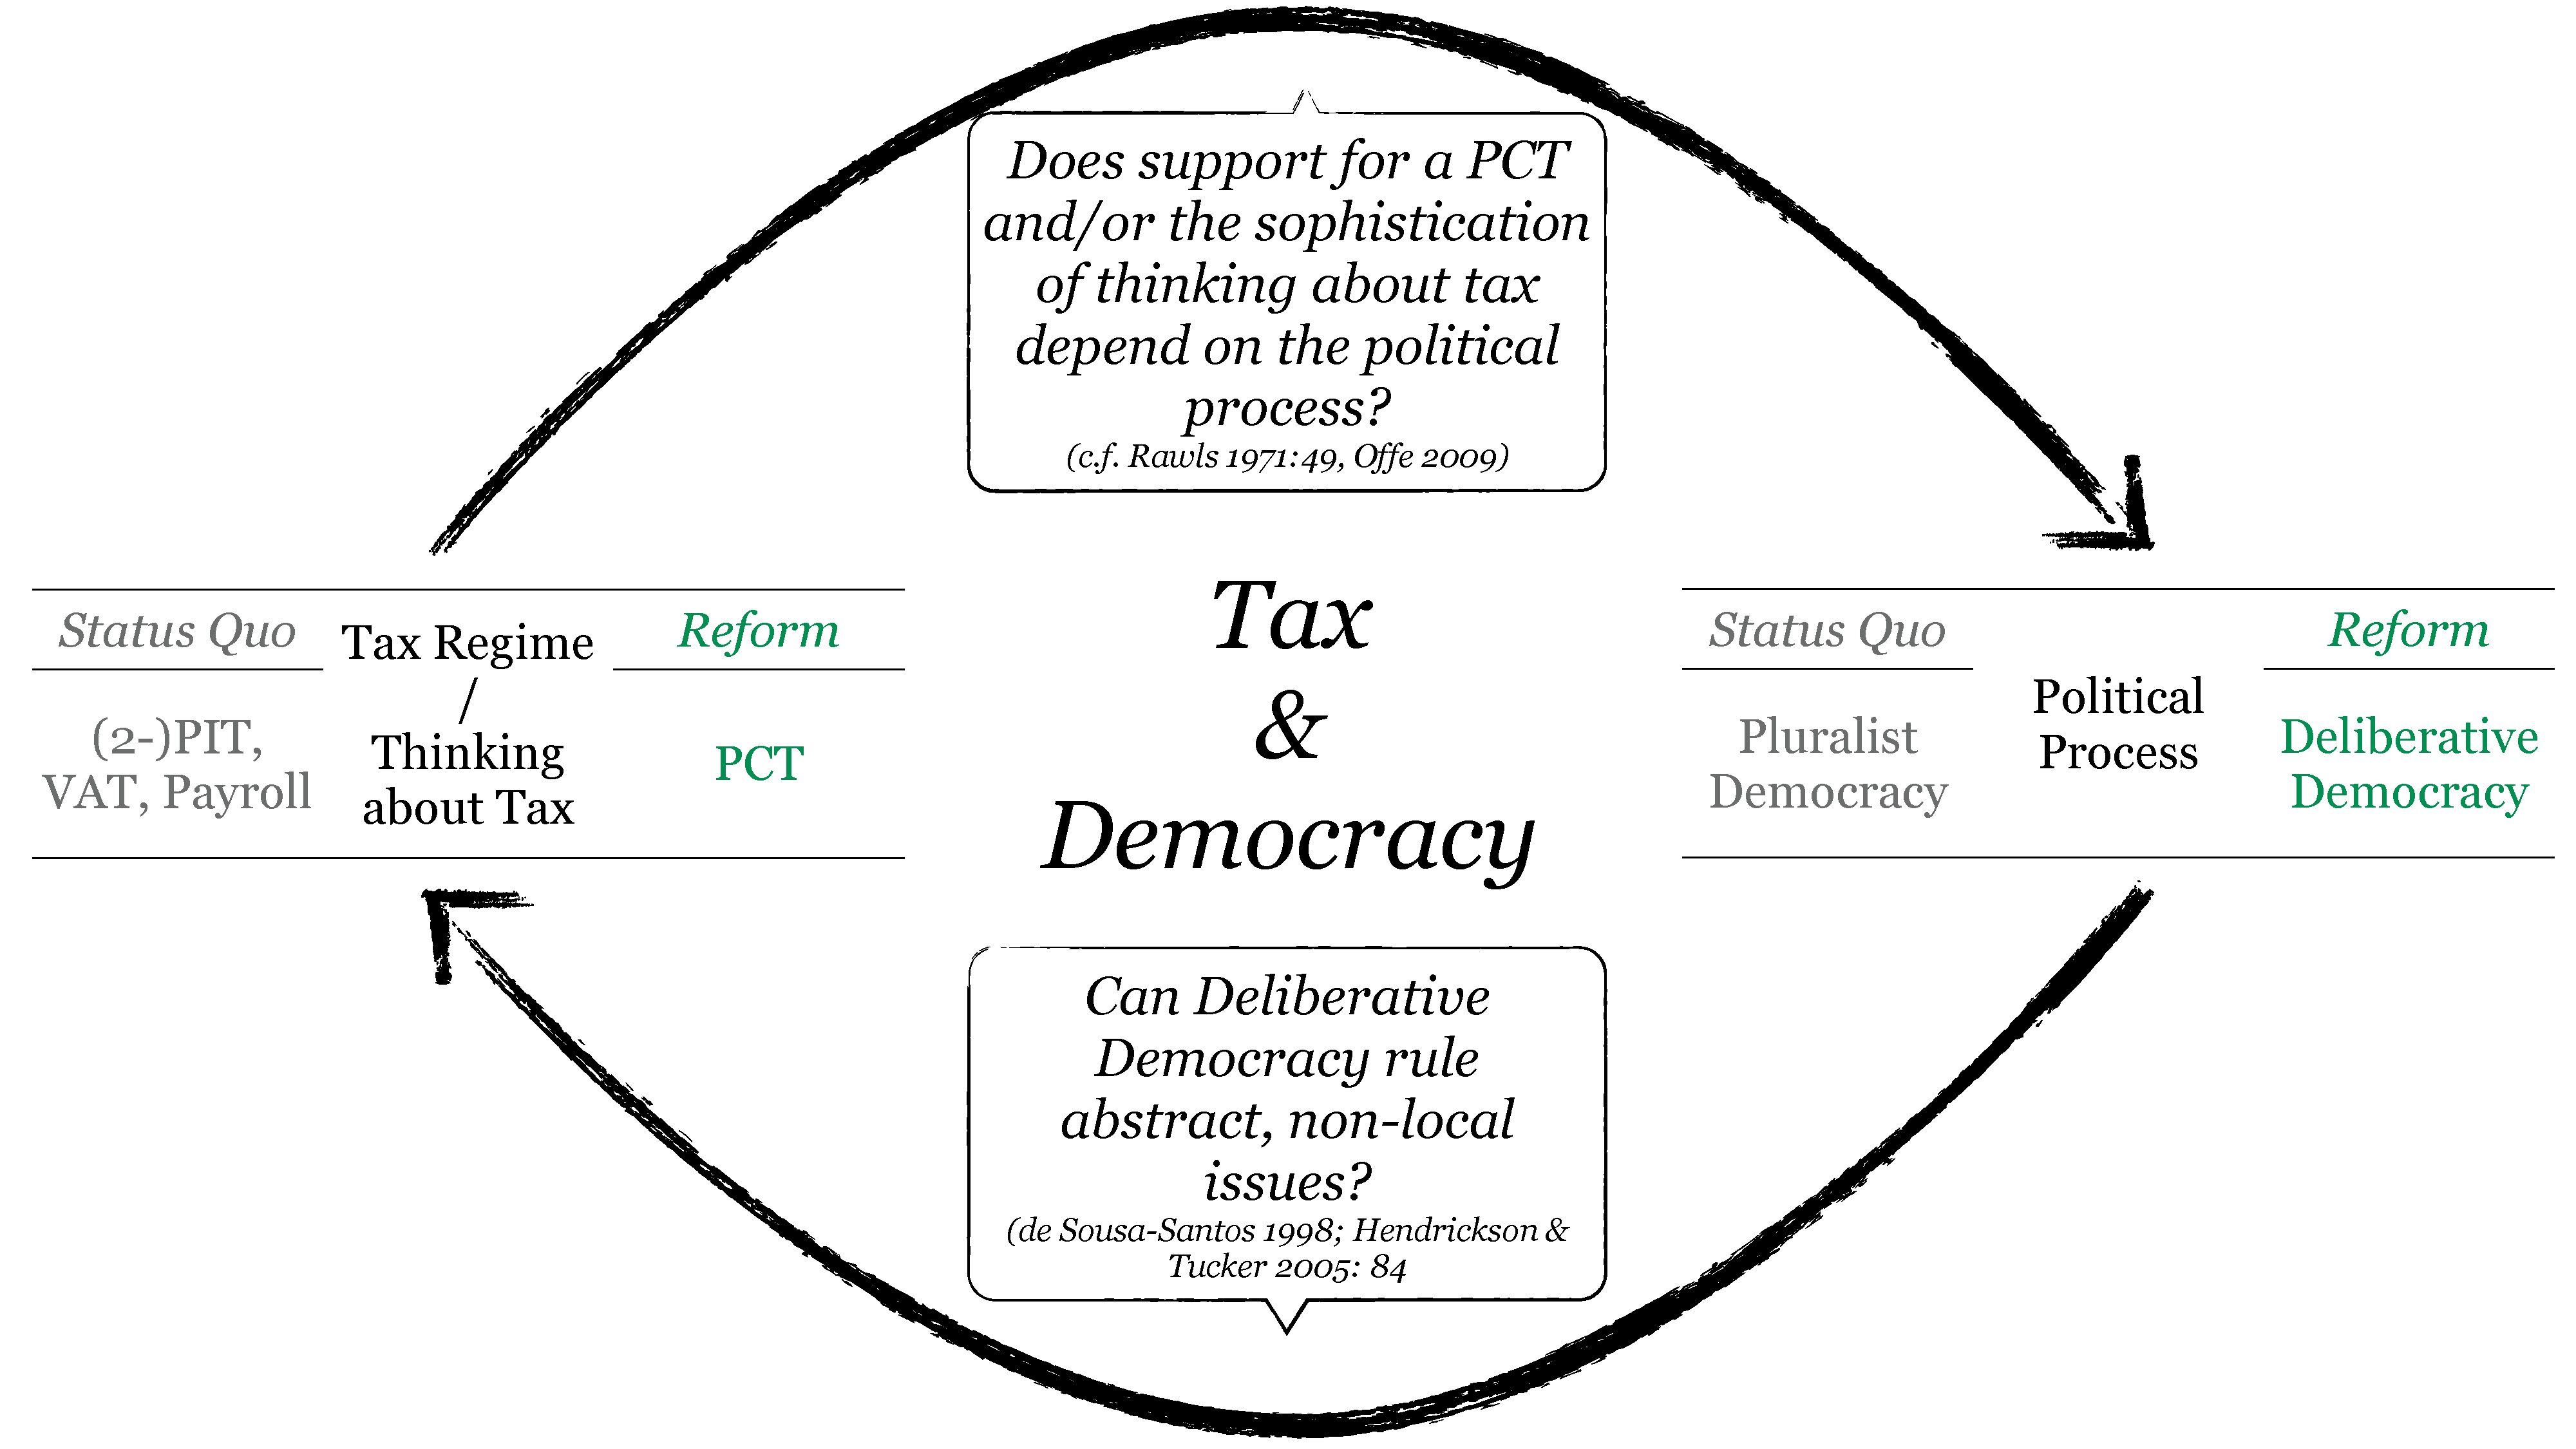
\includegraphics[width=1\linewidth]{tax-democracy}
	\caption{Taxation and Democracy}
	\label{fig:tax-democracy}
\end{figure}

Surely, such a broadly defined research agenda risks hubris, but it also promises to formulate and maybe, tentatively answer some important questions for the social sciences.
I may well --- figuratively --- be biting off more than I can chew, and it sometimes shows (for example in \autoref{chap:wanted}).
All I can do is to tentatively mull over a mouthful at a time, and spit out again that which I cannot address.
This --- forgive the metaphor --- \emph{rumination} takes a lot of pages to write and read, but at least, it is a relatively transparent way of reasoning.
Maybe, in the spirit of Umberto Eco's \emph{anti-library} \citep[as recounted in][]{Taleb2007}, explicating what I do not know or cannot address in this dissertation will make for better questions.
\footnote{
	For this comparison, I am indebted to Maike Schulz, who --- citing Eco --- reminded me in 2013 that an ever elongating reading list need not be a bad thing.
}
Still, to digest anything in full, I must concentrate.
Counterintuitively, the often economic or even technical abstractions of taxation and public choice provide a great guide here.
This mostly \emph{a priori} knowledge, too, requires a lot of pages to write and to read, but, akin to enzymes in the digestive tract, it helps me break down complex issues to ever simpler, fewer and clearer questions (as in \autoref{chap:mixed-economy} and \autoref{part:tax}) that can be handily metabolized into a new, and hopefully original argument that I put to the test.

Admittedly, too, underlying this research are normative convictions about political and economic opportunity, and even human destiny.
Somehow, such a prescriptive impetus has become unacceptable in much of (German) social science on the welfare state.
I must indeed avoid ``politics-based evidence making'' (The Economist, 2012) %add correct reference
or any other conflation of what should be, with what is.
However, even from a merely positive perspective, and even to readers who may not agree with these convictions, the hypotheticals they raise pose analytically worthy questions:
If there is indeed another, superior fiscal configuration on which we could democratically agree --- but do not --- this absence needs explaining.

If anything, finding that which needs a social explanation, must be a worthwhile attempt for the social sciences.

It, too, is how social sciences can contribute to human progress, by \emph{politicizing} the status quo.
\begin{quote}
	``Politicization is the realization that established social norms, social practices, and social relations are contingent rather than sacrosanct, that things could also be different and that citizens, individual and collectively, have political agency by means of which alternatives can be explored and implemented.
	This recognition that things could also be different has always been the igniting spark of the emancipatory-progressive movements, and politicization has always been their key strategy.''
	\\*
 	--- \citet[313]{Bluhdorn-2007-aa}
 	%add first name
\end{quote}

%If risky, this thesis has substantial analytical potential.
%This thesis illuminates the crucial, but so far underinvestigated link between democratic process and tax regime choice.
%It informs the pressing question of the sustainability of the welfare state.
%On the other hand, it tests the ability of deliberative fora to rule on matters of great complexity and large scope.
%If the experimental deliberative forum rules in favor of the PCT, it will have passed a strong test of democratic legitimacy.

%But \hyperref[sec:Wanted]{the question} can probably be answered in the negative:
%no, this is not the best of all liberal-democratic, capitalist and open worlds.

%This desirable, doable hypothetical of the perfect tax demands political science explanations:
%why are we not doing better?
% why do we settle for a structurally underfunded polity in an otherwise prosperous era?
%Why do we allow a scourge of structural unemployment to befall millions, deprived and forced into idleness?
%Why do we leave unchecked the positional excesses of our economies, in spite of the better, fairer angels of our nature?

%what's the second order theory?
%It is not an empirical question in any traditional, positivist meaning of the concept, even though it involves complex and multiple empirical assumptions and causal arguments.
%It is argued in the above, why, even from an analytical and empirical, if not entirely disinterested standpoint, said daydreaming is helpful.

%Even leaving normative considerations aside, as I have tried to demonstrate in the above, just academic rigor alone requires us to hypothesize a hypothetical of a globalized, uniformly taxed world economy.
%\subsubsection{Research Question a):
%Is it the Perfect Tax?} Research question a) is a question of normative considerations, based on which a hypothetical engineering of public policy takes place.

%\begin{description}
%	\item{\textbf{Normative Hypothetical are Needed}} Broadly speaking, it is hypothesized that, employing of a normative hypothetical in the investigation of welfare retrenchment will provide analytical added value.
%A concrete and approximately modeled alternative configuration of international tax harmonization will bring the issue into sharper focus.

%\subsection{Plan of the Thesis} Substantial groundwork is required for the bold claims I make in this thesis.
%The merits of the PCT will stand out when fundamental desiderata of taxation are thoroughly discussed.
%Conversely, the demerits of the current fiscal configuration will appear.
%To see clearly through the ``analytic muddle of tax'' (\citealt{McCaffery2005}:
%862) I have to zoom out, establish some abstractions, dynamics and norms of welfare, allocation and inequality seemingly remote to any worldly tax reform.
%They are not.

	%here's the beauty.
%I get to do an empirical work.
%I make this FALSIFIABLE.

%What's the result?
%What happens then?
% pluralism
%delta in attitudes, knowledge etc.
%theory building, critical analysis
%Deliberative Democracy:
%is interest out?
%(yes!)

%Generally, note the Rawlsian, or theory-driven case selection (saturation sampling) backup to representativenss.
%It's not about aggregation.

%4) Can the PCT be implemented nationally?
%That is important for the Deliberative Poll.

%Remember, however, that you don't need perfect absence of prejudice or inequality or ideal speech.
%You just need spech that's a little better than pluralist speech, and a little better than markets.
%Just like Caplan's argument.(this also in response to sanders)

% * step back carefully from my assumptions:
%even if you don't agree with the politics (redistributive and axiomatic in terms of positional spending) of the pct, you've gotta agree with the efficiency.
 %  * even if you don't agree with the PCT, you've gotta agree with the questions it poses.

%Ich hoffe so dem pluralistischen Steuerdiskurs einen (jedenfalls näherungsweise Habermas'schen) Diskurs gegenüber stellen zu können.
%Sollten sich, wie ich annehme, zwischen diesen beiden qualitativen Daten systematische Unterschiede im (Miss)verständnis von Steuer heraus stellen, könnte ich erste Hypothesen über den Zusammenhang von politischem Prozess/Ideal (pluralistisch vs.\ deliberativ/Habermas) und polit-ökonomischem Diskurs ableiten

%I want to (qualitatively) compare the thinking about tax in two very different samples:
%a) expert interviews (politicians, lobbyists) and b) a deliberative jury of randomly selected citizens (Cohen, cf.~Habermas).
%My data will be the discussions in these two samples.
%I assume these samples to reflect two paradigmatic (most different) democratic fora or processes, onepluralist (experts aka.
%interest group reps) one deliberative (jury members).
%My "hypothesis" (I know I'm not supposed to have a hypothesis, this will be an inductive/qualitative endeavour) is that these two democratic fora will differ systematically in the kind of thinking about tax and redistribution that they produce.

%.
%My 2nd order theory of tax is democracy.
%My 2nd order theory of democracy is inequality.
%Offe says:
%write a Konflikttheorie, a 2nd order theory on the reform suggestion (such as Offe 2009)

%Explain how the empirical, testable approach would look.
%But point out:
%there needs to be a plan B, paddle back from this.
%For normative (Cervantes) reasons but also because these are stupid shorthand understandings.

	%overview of what is to come;
%next chapters
%And what kind of research design is this?
%(it's an extreme case)

%\section{Schedule}

	%There is a vibrant and innovative community of scholars and activists who host and moderate deliberative fora of varying designs, particularly in the US.
%Organizing successful deliberations is at least as much an art as a science and requires extensive experience.
%In addition, I must prevent my analytical and normative preoccupation with a particular reform proposal (a postpaid PCT) from exerting undue influence on the deliberation.
%The deliberative must not be set up to confirm the PCT.
%Both hypothesis a) and b) must be falsifiable in this design.
%A postpaid PCT must be presented as one of the (few) fundamental choices in redistributive design.
	%My prior work (Held 2010) on the postpaid PCT can serve as a survey of the trade-offs and desiderata (see summary above) in redistributive design.
%These may serve to organize the expected transformation of previously “amalgamated” (Miller 1992:
%4ff) preferences into distinct, single-peaked dimensions.
% The trade-offs and desiderata are also inputs for questionnaire design and may be used to draft briefing materials.
	%This quasi-experimental design requires great methodological care and experience.
% Ideally,  I will be able to co-host, or investigate a Deliberative Poll ® on redistributive design in Germany or the US, with help from James S.
%Fishkin and the Stanford-based Center for Deliberative Democracy.
% This would ensure rigorous institutional design, peer-reviewed balance and experienced implementation, but requires substantial external (to BIGSSS) funding.
%Should I be unable to secure such funding, some scaled-down version will also be possible.


%%%
\section{Operationalization}

%\cite{Johnson1998}
	%161:
%``Would-be political reformers of various persuasions urge deliberation upon us.
%Yet in their pleadings such theorists and reformers frequently invoke deliberation in an uncritical manner.
%They proceed as though the ways in which deliberation and the effects we can expect of it are not just obvious, but attractively so.''

%\cite{Azmanova2010} (also \cite{Fishkin2009}:
%529)
	%49:
%thoughtfulness and reflexivity (as per Fishkin) require 1) reasonably accurate information 2) substantive balance 3) diversity, 4) conscientiousness, 5) equal consideration

%\cite{Citizen-2004-aa}
	%11:
%one guy did the learning sessions
	%1) has a selection phase
	%2)  has a LEARNING phase
		%also develop "shared values" about the process
	%3) has a PUBLIC HEARING phase
	%4) has a DELIBERATION phase
	%go to church with group, maybe.

%\cite{Dienel-1999-aa}
	%"To make a Planning Cell project go effectively, one needs a process of more than four days.
%We can distinguish five phases:
%design, preparation, implementation, compiling the documentation, follow up.
%After the joint formulation of the task, two problems have to be solved in the second phase:
%The issue has to be translated into a program of 16 work units and the jurors have to be selected and invited.
%Building the program is crucial for the Planning Cell preparation.
%Each working unit has to have its clearly defined remit.
%Problems have to be reduced to comprehensible alternatives.
%All this is done by the programmer who is much more important than the moderator''

%\cite{Fung-2003-ac}
	%very good summary, get back to this

%\cite{Fishkin2009}
	%democracies are supposed to fulfill two values;
%political equality and deliberation (K84)
	%``a democracy in which we all had substantive information [and] [\ldots] substantive opinions would seem to take too many meetings.''
	%what's wrong with unenlightened opinions (all K113ff)
		%\begin{enumerate}
			%\item they may be volatile (cite other sources
			%\item people may be manipulated by foregrounding some information (clean coal vs.\ dirty coal, forgetting about natural gas -- compare this to tax choice)
			%\item misinformation (savings rate)
			%\item favor favorable, true arguments over others
			%\item manipulation may ``prime'' one aspect of policy.
		%\end{enumerate}
	%K260:
%``the hard choice, in other words, is between debilitated but actual opinion, on the one hand, and deliberative but counterfactual opinion, on the other.''
	%K369:
%table with raw/refined opinion, and different kinds of sampling.
	%K438:
%``The idea is that if a counterfactual situation is morally relevant, why not do a serious social science experiment -- rather than merely engage in informal inference or armchair empiricism -- to determine what the appropriate counterfactual situation might look like?
%and if that counterfactual is both discoverable and normatively relevent, why not then let the rest of the world know about it?
%Just as John Rawls's original position can be thought of having a kind of recommending force, the counterfactual representation of public opinion identified by the Deliberative Poll also recommends to the rest of the population some conclusions that they ought to take seriously.''
	%K390:
%self-selected samples will be very limited in what they can achieve.
	%K401:
%citizen juries use quota samples, consesus conferences use self-selected samples, then with some quota sampling
	%K550:
%notes that positions must not merely be balanced in terms of airtime or affect, but ``whether the considerations offered in favor of, or against, a proposal, candidate or policy are answered in a substantive way by those who advocate a different position.''
	%K561:
%three categories for such considerations
		%``the benefits or burdens of a policy or political choice,
		% the causal arguments about whether those benefits or benefits or burdens will actually result from one choice or another,
		%and the values by which those benefits and burdens might best be evaluated.''
		%K1424:
%``the problem is that any microcosmis deliberation taking place in a modern society will be one in which there are significant social and economic inequalities in the conduct of ordinary life in the broader society.
		 	%It seems difficult or impossible to `bracket' these inequalities -- for participants to behave `as if' they do not exist.
		 	%Indeed the problem goes deeper.
%The possibility of doing so is the challenge of the ``autonomy of the political'', namely, whether or not equality can hold sway in politics in a world in which inequality rules in economic and social relations.
		 	%The viability and legitimacy of the liberal-democratic process may turn on the answer.''
		 	%notes that the relation between ideal theory and actual practice is ``aspirational'' \citep[K2679]{Fishkin2009}


%\cite{GutmannThompson-2004-aa}
	%loc177:
%`your fellow citizens must give reasons that are comprehensible to you''
	%K188:
%they introduce first and second-order theories, too!
	%K919, writing about Fish:
%``Giving reasons is the chief way of academics to exercise power in democratic politics.
%All the talk about deliberation, like deliberation itself, is merely a cover for power politics.''.

%cite the sausgruber tyran stuff.

%iris marion young, especially notes that people of lower status may have a hard time getting listened to, or that others may be particularly accustomed to orderly forms of reason-giving arguments that weigh with other participants -- and this may be particulary problematic the more substantive the topic is.

%note that

%groupthink!

%tax allows only very limited choice:
%income, consumption or assets;
%a couple of schedules, plus some pigouvian taxation.
% the CIT, notably, is just a special way to raise the PIT.
%Otherwise, only natural persons.
%Tax demands these choices.
%Also, these choices \emph{are} as I explain in the below, political, so they must be made legitimately, and we may not be able to simply outsource them to elites.

%argue exactly why small sub-issues of tax do not work;
%they violate the real choices.

%there remain problems:
%you can't just go about this as if it wwere not controversial;
%it is controversially maongst experts, but more importantly, controversial whether experts have in fact authority and the right context.
%It can't just be an experiment, or a treatment intervention where ordinary citizens must necessarily become more like experts, and if they are not, then the teaching has failed.
%It must be possible for people to disagree with the abstractions they ar epresented with, see the criticism of it.

%tax is very technocratic, simply because the instition is like that.
%this will have to be qualitative
%\end{enumerate}